% Options for packages loaded elsewhere
\PassOptionsToPackage{unicode}{hyperref}
\PassOptionsToPackage{hyphens}{url}
%
\documentclass[
]{article}
\usepackage{amsmath,amssymb}
\usepackage{iftex}
\ifPDFTeX
  \usepackage[T1]{fontenc}
  \usepackage[utf8]{inputenc}
  \usepackage{textcomp} % provide euro and other symbols
\else % if luatex or xetex
  \usepackage{unicode-math} % this also loads fontspec
  \defaultfontfeatures{Scale=MatchLowercase}
  \defaultfontfeatures[\rmfamily]{Ligatures=TeX,Scale=1}
\fi
\usepackage{lmodern}
\ifPDFTeX\else
  % xetex/luatex font selection
\fi
% Use upquote if available, for straight quotes in verbatim environments
\IfFileExists{upquote.sty}{\usepackage{upquote}}{}
\IfFileExists{microtype.sty}{% use microtype if available
  \usepackage[]{microtype}
  \UseMicrotypeSet[protrusion]{basicmath} % disable protrusion for tt fonts
}{}
\makeatletter
\@ifundefined{KOMAClassName}{% if non-KOMA class
  \IfFileExists{parskip.sty}{%
    \usepackage{parskip}
  }{% else
    \setlength{\parindent}{0pt}
    \setlength{\parskip}{6pt plus 2pt minus 1pt}}
}{% if KOMA class
  \KOMAoptions{parskip=half}}
\makeatother
\usepackage{xcolor}
\usepackage[margin=1in]{geometry}
\usepackage{color}
\usepackage{fancyvrb}
\newcommand{\VerbBar}{|}
\newcommand{\VERB}{\Verb[commandchars=\\\{\}]}
\DefineVerbatimEnvironment{Highlighting}{Verbatim}{commandchars=\\\{\}}
% Add ',fontsize=\small' for more characters per line
\usepackage{framed}
\definecolor{shadecolor}{RGB}{248,248,248}
\newenvironment{Shaded}{\begin{snugshade}}{\end{snugshade}}
\newcommand{\AlertTok}[1]{\textcolor[rgb]{0.94,0.16,0.16}{#1}}
\newcommand{\AnnotationTok}[1]{\textcolor[rgb]{0.56,0.35,0.01}{\textbf{\textit{#1}}}}
\newcommand{\AttributeTok}[1]{\textcolor[rgb]{0.13,0.29,0.53}{#1}}
\newcommand{\BaseNTok}[1]{\textcolor[rgb]{0.00,0.00,0.81}{#1}}
\newcommand{\BuiltInTok}[1]{#1}
\newcommand{\CharTok}[1]{\textcolor[rgb]{0.31,0.60,0.02}{#1}}
\newcommand{\CommentTok}[1]{\textcolor[rgb]{0.56,0.35,0.01}{\textit{#1}}}
\newcommand{\CommentVarTok}[1]{\textcolor[rgb]{0.56,0.35,0.01}{\textbf{\textit{#1}}}}
\newcommand{\ConstantTok}[1]{\textcolor[rgb]{0.56,0.35,0.01}{#1}}
\newcommand{\ControlFlowTok}[1]{\textcolor[rgb]{0.13,0.29,0.53}{\textbf{#1}}}
\newcommand{\DataTypeTok}[1]{\textcolor[rgb]{0.13,0.29,0.53}{#1}}
\newcommand{\DecValTok}[1]{\textcolor[rgb]{0.00,0.00,0.81}{#1}}
\newcommand{\DocumentationTok}[1]{\textcolor[rgb]{0.56,0.35,0.01}{\textbf{\textit{#1}}}}
\newcommand{\ErrorTok}[1]{\textcolor[rgb]{0.64,0.00,0.00}{\textbf{#1}}}
\newcommand{\ExtensionTok}[1]{#1}
\newcommand{\FloatTok}[1]{\textcolor[rgb]{0.00,0.00,0.81}{#1}}
\newcommand{\FunctionTok}[1]{\textcolor[rgb]{0.13,0.29,0.53}{\textbf{#1}}}
\newcommand{\ImportTok}[1]{#1}
\newcommand{\InformationTok}[1]{\textcolor[rgb]{0.56,0.35,0.01}{\textbf{\textit{#1}}}}
\newcommand{\KeywordTok}[1]{\textcolor[rgb]{0.13,0.29,0.53}{\textbf{#1}}}
\newcommand{\NormalTok}[1]{#1}
\newcommand{\OperatorTok}[1]{\textcolor[rgb]{0.81,0.36,0.00}{\textbf{#1}}}
\newcommand{\OtherTok}[1]{\textcolor[rgb]{0.56,0.35,0.01}{#1}}
\newcommand{\PreprocessorTok}[1]{\textcolor[rgb]{0.56,0.35,0.01}{\textit{#1}}}
\newcommand{\RegionMarkerTok}[1]{#1}
\newcommand{\SpecialCharTok}[1]{\textcolor[rgb]{0.81,0.36,0.00}{\textbf{#1}}}
\newcommand{\SpecialStringTok}[1]{\textcolor[rgb]{0.31,0.60,0.02}{#1}}
\newcommand{\StringTok}[1]{\textcolor[rgb]{0.31,0.60,0.02}{#1}}
\newcommand{\VariableTok}[1]{\textcolor[rgb]{0.00,0.00,0.00}{#1}}
\newcommand{\VerbatimStringTok}[1]{\textcolor[rgb]{0.31,0.60,0.02}{#1}}
\newcommand{\WarningTok}[1]{\textcolor[rgb]{0.56,0.35,0.01}{\textbf{\textit{#1}}}}
\usepackage{graphicx}
\makeatletter
\def\maxwidth{\ifdim\Gin@nat@width>\linewidth\linewidth\else\Gin@nat@width\fi}
\def\maxheight{\ifdim\Gin@nat@height>\textheight\textheight\else\Gin@nat@height\fi}
\makeatother
% Scale images if necessary, so that they will not overflow the page
% margins by default, and it is still possible to overwrite the defaults
% using explicit options in \includegraphics[width, height, ...]{}
\setkeys{Gin}{width=\maxwidth,height=\maxheight,keepaspectratio}
% Set default figure placement to htbp
\makeatletter
\def\fps@figure{htbp}
\makeatother
\setlength{\emergencystretch}{3em} % prevent overfull lines
\providecommand{\tightlist}{%
  \setlength{\itemsep}{0pt}\setlength{\parskip}{0pt}}
\setcounter{secnumdepth}{-\maxdimen} % remove section numbering
\ifLuaTeX
  \usepackage{selnolig}  % disable illegal ligatures
\fi
\IfFileExists{bookmark.sty}{\usepackage{bookmark}}{\usepackage{hyperref}}
\IfFileExists{xurl.sty}{\usepackage{xurl}}{} % add URL line breaks if available
\urlstyle{same}
\hypersetup{
  pdftitle={HUDM6052 Psychometric II Homework\_01},
  pdfauthor={Chenguang Pan (cp3280@tc.columbia.edu)},
  hidelinks,
  pdfcreator={LaTeX via pandoc}}

\title{HUDM6052 Psychometric II Homework\_01}
\author{Chenguang Pan
(\href{mailto:cp3280@tc.columbia.edu}{\nolinkurl{cp3280@tc.columbia.edu}})}
\date{2023-09-28}

\begin{document}
\maketitle

\setcounter{tocdepth}{4}
\tableofcontents

\hypertarget{q1-parta}{%
\subsection{Q1-Part(a)}\label{q1-parta}}

\emph{Plot the following two items using the normal ogive model over the
range..}

\textbf{My Solution: }

First, I define the normal ogive model.

\begin{Shaded}
\begin{Highlighting}[]
\SpecialCharTok{\textgreater{}} \CommentTok{\# define the theta}
\ErrorTok{\textgreater{}}\NormalTok{ theta }\OtherTok{\textless{}{-}} \FunctionTok{seq}\NormalTok{(}\SpecialCharTok{{-}}\DecValTok{3}\NormalTok{,}\DecValTok{3}\NormalTok{, }\AttributeTok{by=}\FloatTok{0.1}\NormalTok{)}
\SpecialCharTok{\textgreater{}} 
\ErrorTok{\textgreater{}} \CommentTok{\# define the normal ogive model}
\ErrorTok{\textgreater{}}\NormalTok{ nom\_2pl }\OtherTok{\textless{}{-}} \ControlFlowTok{function}\NormalTok{(theta, a, b)\{}
\SpecialCharTok{+}   \CommentTok{\# get the probit vector}
\SpecialCharTok{+}\NormalTok{   Z }\OtherTok{\textless{}{-}}\NormalTok{ a}\SpecialCharTok{*}\NormalTok{(theta}\SpecialCharTok{{-}}\NormalTok{b)}
\SpecialCharTok{+}\NormalTok{   func\_ }\OtherTok{\textless{}{-}} \ControlFlowTok{function}\NormalTok{(probit)\{(}\DecValTok{1}\SpecialCharTok{/}\FunctionTok{sqrt}\NormalTok{(}\DecValTok{2}\SpecialCharTok{*}\NormalTok{pi))}\SpecialCharTok{*}\FunctionTok{exp}\NormalTok{(}\SpecialCharTok{{-}}\FloatTok{0.5}\SpecialCharTok{*}\NormalTok{probit}\SpecialCharTok{\^{}}\DecValTok{2}\NormalTok{)\}}
\SpecialCharTok{+}\NormalTok{   p\_list }\OtherTok{\textless{}{-}} \FunctionTok{c}\NormalTok{()}
\SpecialCharTok{+}   \CommentTok{\# using a for loop to get the p iteratively}
\SpecialCharTok{+}   \ControlFlowTok{for}\NormalTok{ (i }\ControlFlowTok{in} \DecValTok{1}\SpecialCharTok{:}\FunctionTok{length}\NormalTok{(Z)) \{}
\SpecialCharTok{+}     \CommentTok{\# get the CDF}
\SpecialCharTok{+}\NormalTok{     p\_i }\OtherTok{\textless{}{-}} \FunctionTok{integrate}\NormalTok{(func\_, }\SpecialCharTok{{-}}\NormalTok{Z[i], }\ConstantTok{Inf}\NormalTok{)}
\SpecialCharTok{+}     \CommentTok{\# store the result}
\SpecialCharTok{+}\NormalTok{     p\_list[i] }\OtherTok{\textless{}{-}}\NormalTok{ p\_i}
\SpecialCharTok{+}\NormalTok{   \}}
\SpecialCharTok{+}   \FunctionTok{return}\NormalTok{(p\_list)}
\SpecialCharTok{+}\NormalTok{ \}}
\end{Highlighting}
\end{Shaded}

Then, using the function above to plot the ICCs for two items.\\
For the item 1 with \(\alpha=1\) and \(\beta =1\).

\begin{Shaded}
\begin{Highlighting}[]
\SpecialCharTok{\textgreater{}} \CommentTok{\# Item 1: a=1, b=1}
\ErrorTok{\textgreater{}} \CommentTok{\# define the xlim}
\ErrorTok{\textgreater{}}\NormalTok{ xlim\_min }\OtherTok{\textless{}{-}} \SpecialCharTok{{-}}\DecValTok{3}
\SpecialCharTok{\textgreater{}}\NormalTok{ xlim\_max }\OtherTok{\textless{}{-}} \DecValTok{3}
\SpecialCharTok{\textgreater{}}\NormalTok{ P\_item1\_nom }\OtherTok{\textless{}{-}} \FunctionTok{nom\_2pl}\NormalTok{(}\AttributeTok{theta=}\NormalTok{theta,}\AttributeTok{a=}\DecValTok{1}\NormalTok{,}\AttributeTok{b=}\DecValTok{1}\NormalTok{)}
\SpecialCharTok{\textgreater{}} \FunctionTok{plot}\NormalTok{(theta, P\_item1\_nom, }\AttributeTok{type =} \StringTok{"l"}\NormalTok{, }
\SpecialCharTok{+}      \AttributeTok{col=}\StringTok{"red"}\NormalTok{, }\AttributeTok{xlim =} \FunctionTok{c}\NormalTok{(xlim\_min,xlim\_max), }\AttributeTok{ylim =} \FunctionTok{c}\NormalTok{(}\DecValTok{0}\NormalTok{,}\DecValTok{1}\NormalTok{),}
\SpecialCharTok{+}      \AttributeTok{main =} \StringTok{"Item 1, a=1, b=1"}\NormalTok{, }\AttributeTok{ylab =} \StringTok{"P(theta)"}\NormalTok{)}
\SpecialCharTok{\textgreater{}} 
\ErrorTok{\textgreater{}} \CommentTok{\# add a horizontal line at p=0.5 to see the b value}
\ErrorTok{\textgreater{}} \FunctionTok{abline}\NormalTok{(}\AttributeTok{h=}\FloatTok{0.5}\NormalTok{, }\AttributeTok{col=}\StringTok{"blue"}\NormalTok{, }\AttributeTok{lty=}\DecValTok{2}\NormalTok{)}
\SpecialCharTok{\textgreater{}} \FunctionTok{abline}\NormalTok{(}\AttributeTok{v=}\DecValTok{1}\NormalTok{, }\AttributeTok{col=}\StringTok{"blue"}\NormalTok{, }\AttributeTok{lty=}\DecValTok{2}\NormalTok{)}
\SpecialCharTok{\textgreater{}} \FunctionTok{grid}\NormalTok{()}
\end{Highlighting}
\end{Shaded}

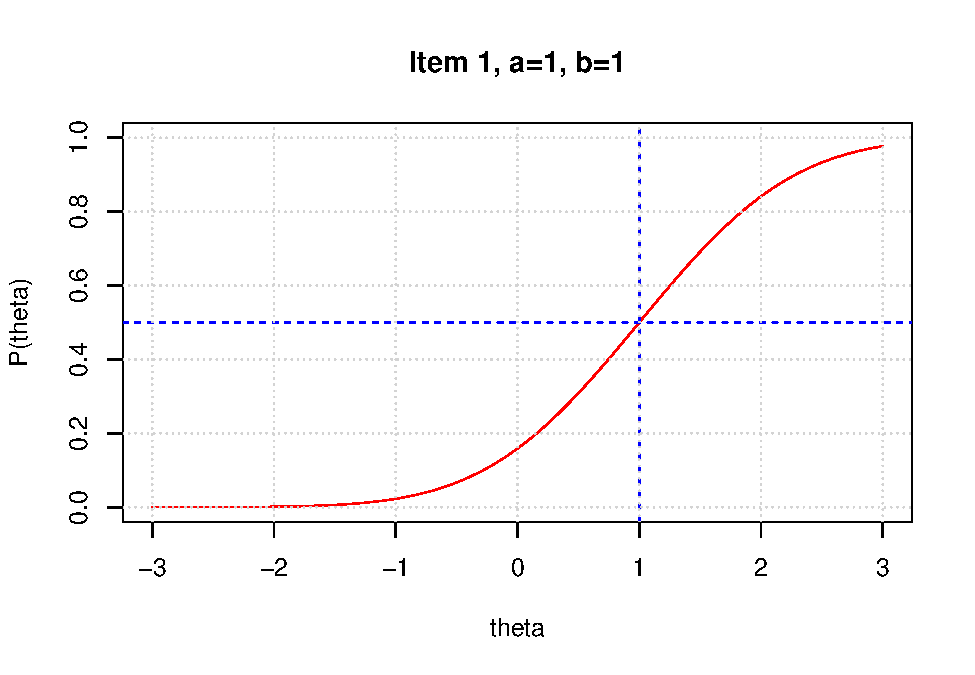
\includegraphics[width=1\linewidth,height=0.5\textheight]{Assignment_1_files/figure-latex/unnamed-chunk-2-1}

For the Item 2 with \(\alpha=.5957\) and \(\beta=-0.5\).

\begin{Shaded}
\begin{Highlighting}[]
\SpecialCharTok{\textgreater{}} \CommentTok{\# Item 1: a=.5957, b={-}.5}
\ErrorTok{\textgreater{}} \CommentTok{\# par(mfrow=c(1,2))}
\ErrorTok{\textgreater{}}\NormalTok{ P\_item2\_nom }\OtherTok{\textless{}{-}} \FunctionTok{nom\_2pl}\NormalTok{(}\AttributeTok{theta=}\NormalTok{theta,}\AttributeTok{a=}\NormalTok{.}\DecValTok{5957}\NormalTok{,}\AttributeTok{b=}\SpecialCharTok{{-}}\FloatTok{0.5}\NormalTok{)}
\SpecialCharTok{\textgreater{}} \FunctionTok{plot}\NormalTok{(theta, P\_item2\_nom, }\AttributeTok{type =} \StringTok{"l"}\NormalTok{, }
\SpecialCharTok{+}      \AttributeTok{col=}\StringTok{"red"}\NormalTok{, }\AttributeTok{xlim =} \FunctionTok{c}\NormalTok{(xlim\_min,xlim\_max), }\AttributeTok{ylim =} \FunctionTok{c}\NormalTok{(}\DecValTok{0}\NormalTok{,}\DecValTok{1}\NormalTok{),}
\SpecialCharTok{+}      \AttributeTok{main =} \StringTok{"Item 2, a=.5957, b={-}0.5"}\NormalTok{, }\AttributeTok{ylab =} \StringTok{"P(theta)"}\NormalTok{)}
\SpecialCharTok{\textgreater{}} 
\ErrorTok{\textgreater{}} \CommentTok{\# add a horizontal line at p=0.5 to see the b value}
\ErrorTok{\textgreater{}} \FunctionTok{abline}\NormalTok{(}\AttributeTok{h=}\FloatTok{0.5}\NormalTok{, }\AttributeTok{col=}\StringTok{"blue"}\NormalTok{, }\AttributeTok{lty=}\DecValTok{2}\NormalTok{)}
\SpecialCharTok{\textgreater{}} \FunctionTok{abline}\NormalTok{(}\AttributeTok{v=}\SpecialCharTok{{-}}\FloatTok{0.5}\NormalTok{, }\AttributeTok{col=}\StringTok{"blue"}\NormalTok{, }\AttributeTok{lty=}\DecValTok{2}\NormalTok{)}
\SpecialCharTok{\textgreater{}} \FunctionTok{grid}\NormalTok{()}
\end{Highlighting}
\end{Shaded}

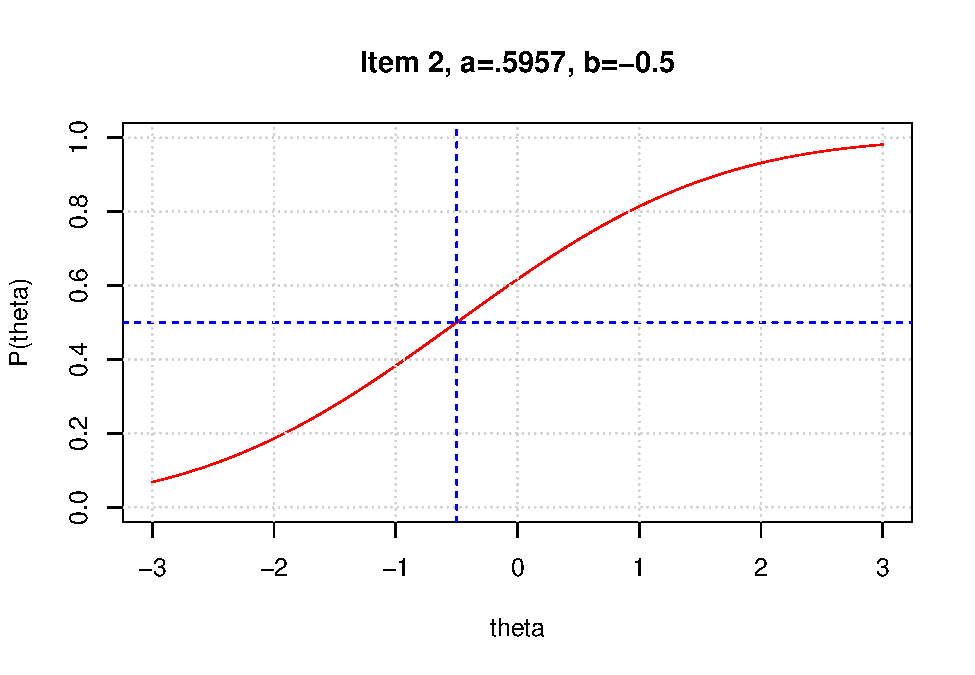
\includegraphics{Assignment_1_files/figure-latex/unnamed-chunk-3-1.pdf}

\hypertarget{q1-partb}{%
\subsection{Q1-Part(b)}\label{q1-partb}}

\emph{Plot the following two items using a logistic model over the
range..}

\textbf{My Solution: }

Like before, I defined the model first. This time, the model is much
simpler.

\begin{Shaded}
\begin{Highlighting}[]
\SpecialCharTok{\textgreater{}}\NormalTok{ logit\_2pl }\OtherTok{\textless{}{-}} \ControlFlowTok{function}\NormalTok{(theta, a, b)\{}
\SpecialCharTok{+}   \CommentTok{\# get the logit}
\SpecialCharTok{+}\NormalTok{   Z }\OtherTok{\textless{}{-}}\NormalTok{ a}\SpecialCharTok{*}\NormalTok{(theta}\SpecialCharTok{{-}}\NormalTok{b)}
\SpecialCharTok{+}   \CommentTok{\# get the probability}
\SpecialCharTok{+}\NormalTok{   P }\OtherTok{\textless{}{-}} \DecValTok{1}\SpecialCharTok{/}\NormalTok{(}\DecValTok{1} \SpecialCharTok{+} \FunctionTok{exp}\NormalTok{(}\SpecialCharTok{{-}}\NormalTok{Z))}
\SpecialCharTok{+}   \FunctionTok{return}\NormalTok{(P)}
\SpecialCharTok{+}\NormalTok{ \}}
\end{Highlighting}
\end{Shaded}

Then, using the function above to plot the ICCs for two items.\\
For the item 1 with \(\alpha=1\) and \(\beta =1\).

\begin{Shaded}
\begin{Highlighting}[]
\SpecialCharTok{\textgreater{}}\NormalTok{ P\_item1\_logit }\OtherTok{\textless{}{-}} \FunctionTok{logit\_2pl}\NormalTok{(}\AttributeTok{theta=}\NormalTok{theta,}\AttributeTok{a=}\DecValTok{1}\NormalTok{,}\AttributeTok{b=}\DecValTok{1}\NormalTok{)}
\SpecialCharTok{\textgreater{}} \FunctionTok{plot}\NormalTok{(theta, P\_item1\_logit, }\AttributeTok{type =} \StringTok{"l"}\NormalTok{, }
\SpecialCharTok{+}      \AttributeTok{col=}\StringTok{"darkgreen"}\NormalTok{,  }\AttributeTok{xlim =} \FunctionTok{c}\NormalTok{(xlim\_min,xlim\_max), }\AttributeTok{ylim =} \FunctionTok{c}\NormalTok{(}\DecValTok{0}\NormalTok{,}\DecValTok{1}\NormalTok{),}
\SpecialCharTok{+}      \AttributeTok{main =} \StringTok{"Item 1, a=1, b=1"}\NormalTok{, }\AttributeTok{ylab =} \StringTok{"P(theta)"}\NormalTok{)}
\SpecialCharTok{\textgreater{}} 
\ErrorTok{\textgreater{}} \CommentTok{\# add a horizontal line at p=0.5 to see the b value}
\ErrorTok{\textgreater{}} \FunctionTok{abline}\NormalTok{(}\AttributeTok{h=}\FloatTok{0.5}\NormalTok{, }\AttributeTok{col=}\StringTok{"blue"}\NormalTok{, }\AttributeTok{lty=}\DecValTok{2}\NormalTok{)}
\SpecialCharTok{\textgreater{}} \FunctionTok{abline}\NormalTok{(}\AttributeTok{v=}\DecValTok{1}\NormalTok{, }\AttributeTok{col=}\StringTok{"blue"}\NormalTok{, }\AttributeTok{lty=}\DecValTok{2}\NormalTok{)}
\SpecialCharTok{\textgreater{}} \FunctionTok{grid}\NormalTok{()}
\end{Highlighting}
\end{Shaded}

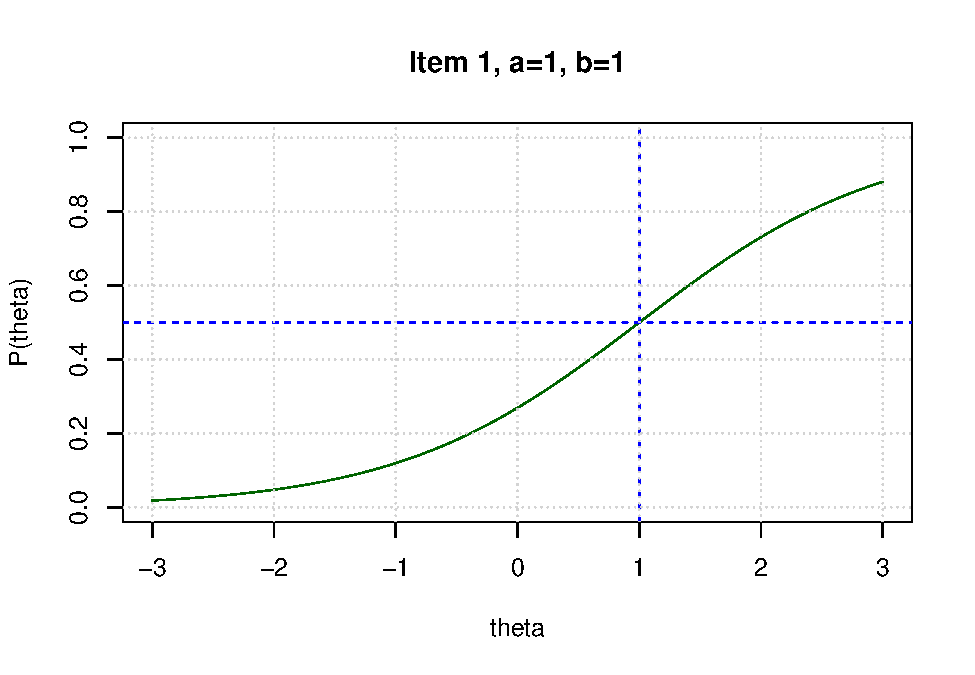
\includegraphics{Assignment_1_files/figure-latex/unnamed-chunk-5-1.pdf}

For the Item 2 with \(\alpha=.5957\) and \(\beta=-0.5\).

\begin{Shaded}
\begin{Highlighting}[]
\SpecialCharTok{\textgreater{}} \CommentTok{\# Item 1: a=.5957, b={-}.5}
\ErrorTok{\textgreater{}} \CommentTok{\# par(mfrow=c(1,2))}
\ErrorTok{\textgreater{}}\NormalTok{ P\_item2\_logit }\OtherTok{\textless{}{-}} \FunctionTok{logit\_2pl}\NormalTok{(}\AttributeTok{theta=}\NormalTok{theta,}\AttributeTok{a=}\NormalTok{.}\DecValTok{5957}\NormalTok{,}\AttributeTok{b=}\SpecialCharTok{{-}}\FloatTok{0.5}\NormalTok{)}
\SpecialCharTok{\textgreater{}} \FunctionTok{plot}\NormalTok{(theta, P\_item2\_logit, }\AttributeTok{type =} \StringTok{"l"}\NormalTok{, }
\SpecialCharTok{+}      \AttributeTok{col=}\StringTok{"darkgreen"}\NormalTok{, }\AttributeTok{xlim =} \FunctionTok{c}\NormalTok{(xlim\_min,xlim\_max), }\AttributeTok{ylim =} \FunctionTok{c}\NormalTok{(}\DecValTok{0}\NormalTok{,}\DecValTok{1}\NormalTok{),}
\SpecialCharTok{+}      \AttributeTok{main =} \StringTok{"Item 2, a=.5957, b={-}0.5"}\NormalTok{, }\AttributeTok{ylab =} \StringTok{"P(theta)"}\NormalTok{)}
\SpecialCharTok{\textgreater{}} 
\ErrorTok{\textgreater{}} \CommentTok{\# add a horizontal line at p=0.5 to see the b value}
\ErrorTok{\textgreater{}} \FunctionTok{abline}\NormalTok{(}\AttributeTok{h=}\FloatTok{0.5}\NormalTok{, }\AttributeTok{col=}\StringTok{"blue"}\NormalTok{, }\AttributeTok{lty=}\DecValTok{2}\NormalTok{)}
\SpecialCharTok{\textgreater{}} \FunctionTok{abline}\NormalTok{(}\AttributeTok{v=}\SpecialCharTok{{-}}\FloatTok{0.5}\NormalTok{, }\AttributeTok{col=}\StringTok{"blue"}\NormalTok{, }\AttributeTok{lty=}\DecValTok{2}\NormalTok{)}
\SpecialCharTok{\textgreater{}} \FunctionTok{grid}\NormalTok{()}
\end{Highlighting}
\end{Shaded}

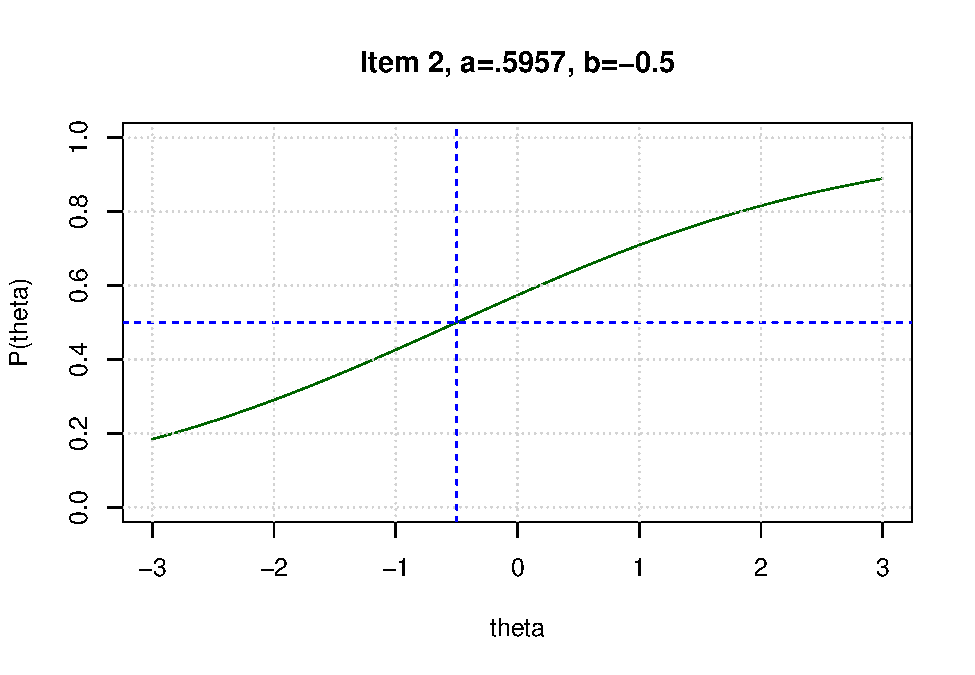
\includegraphics{Assignment_1_files/figure-latex/unnamed-chunk-6-1.pdf}

\hypertarget{q1-partc}{%
\subsection{Q1-Part(c)}\label{q1-partc}}

\emph{Compare the two plots in (b) with the two plots in part (a). What
do you find?..}

\textbf{My Solution: }

For better comparison, I combined the item 1's ICCs from two model, and
so did item 2.\\
ICCs for item 1.

\begin{Shaded}
\begin{Highlighting}[]
\SpecialCharTok{\textgreater{}} \FunctionTok{plot}\NormalTok{(theta, P\_item1\_nom, }\AttributeTok{type =} \StringTok{"l"}\NormalTok{, }
\SpecialCharTok{+}      \AttributeTok{col=}\StringTok{"red"}\NormalTok{, }\AttributeTok{xlim =} \FunctionTok{c}\NormalTok{(xlim\_min,xlim\_max), }\AttributeTok{ylim =} \FunctionTok{c}\NormalTok{(}\DecValTok{0}\NormalTok{,}\DecValTok{1}\NormalTok{),}
\SpecialCharTok{+}      \AttributeTok{main =} \StringTok{"Item 1\textquotesingle{}s ICCs, a=1, b=1"}\NormalTok{, }\AttributeTok{ylab =} \StringTok{"P(theta)"}\NormalTok{)}
\SpecialCharTok{\textgreater{}} \FunctionTok{lines}\NormalTok{(theta, P\_item1\_logit, }\AttributeTok{col=}\StringTok{"green"}\NormalTok{)}
\SpecialCharTok{\textgreater{}} \FunctionTok{abline}\NormalTok{(}\AttributeTok{h=}\FloatTok{0.5}\NormalTok{, }\AttributeTok{col=}\StringTok{"blue"}\NormalTok{, }\AttributeTok{lty=}\DecValTok{2}\NormalTok{)}
\SpecialCharTok{\textgreater{}} \FunctionTok{abline}\NormalTok{(}\AttributeTok{v=}\DecValTok{1}\NormalTok{, }\AttributeTok{col=}\StringTok{"blue"}\NormalTok{, }\AttributeTok{lty=}\DecValTok{2}\NormalTok{)}
\SpecialCharTok{\textgreater{}} \FunctionTok{grid}\NormalTok{()}
\SpecialCharTok{\textgreater{}} \CommentTok{\# add legend}
\ErrorTok{\textgreater{}} \FunctionTok{legend}\NormalTok{(}\StringTok{\textquotesingle{}bottomright\textquotesingle{}}\NormalTok{,}\AttributeTok{inset=}\FloatTok{0.05}\NormalTok{,}
\SpecialCharTok{+}        \FunctionTok{c}\NormalTok{(}\StringTok{"Normal Ogive"}\NormalTok{,}\StringTok{"Logistic"}\NormalTok{),}\AttributeTok{lty=}\DecValTok{1}\NormalTok{,}
\SpecialCharTok{+}        \AttributeTok{col=}\FunctionTok{c}\NormalTok{(}\StringTok{"red"}\NormalTok{,}\StringTok{"green"}\NormalTok{),}\AttributeTok{title=}\StringTok{"Graph type"}\NormalTok{,}
\SpecialCharTok{+}        \AttributeTok{cex=}\FloatTok{0.8}\NormalTok{)}
\end{Highlighting}
\end{Shaded}

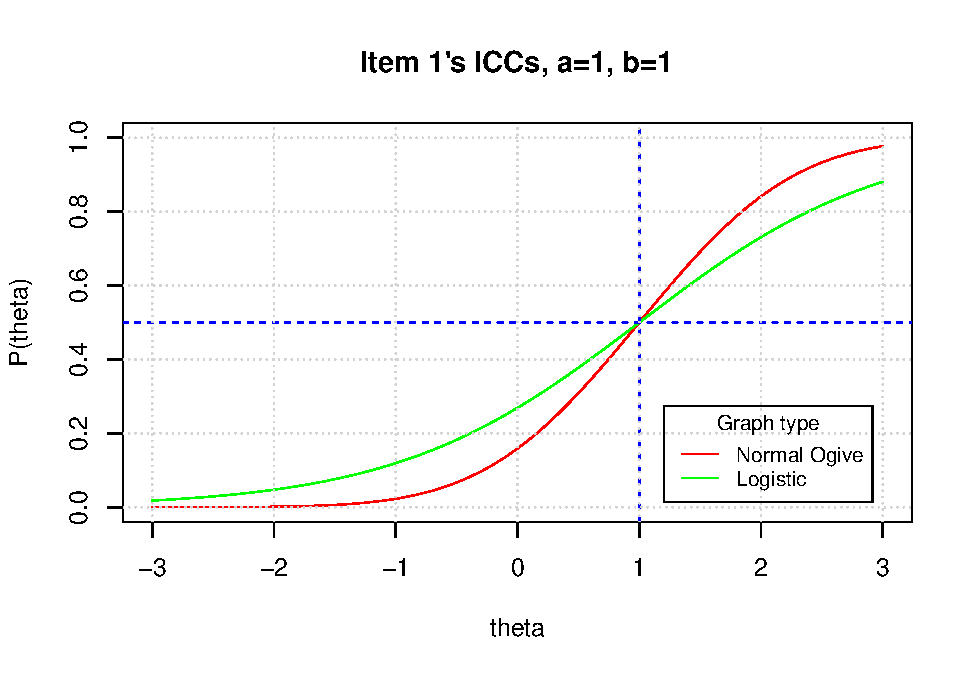
\includegraphics{Assignment_1_files/figure-latex/unnamed-chunk-7-1.pdf}
The plot shows that ICCs intersect at the \(P(\theta) = 0.5\) with a
same corresponding \(\beta = 1\). However, the slope of logistic model's
ICC is lighter than it from the normal ogive model.

Next, I use the converted \(\alpha_c = 1.702\alpha\) to re-plot the
ICCs.

\begin{Shaded}
\begin{Highlighting}[]
\SpecialCharTok{\textgreater{}} \CommentTok{\# adjust the alpha}
\ErrorTok{\textgreater{}}\NormalTok{ P\_item1\_logit }\OtherTok{\textless{}{-}} \FunctionTok{logit\_2pl}\NormalTok{(}\AttributeTok{theta=}\NormalTok{theta,}\AttributeTok{a=}\DecValTok{1}\SpecialCharTok{*}\FloatTok{1.702}\NormalTok{,}\AttributeTok{b=}\DecValTok{1}\NormalTok{)}
\SpecialCharTok{\textgreater{}} \CommentTok{\# replot the two ICCs}
\ErrorTok{\textgreater{}} \FunctionTok{plot}\NormalTok{(theta, P\_item1\_nom, }\AttributeTok{type =} \StringTok{"l"}\NormalTok{, }
\SpecialCharTok{+}      \AttributeTok{col=}\StringTok{"red"}\NormalTok{, }\AttributeTok{xlim =} \FunctionTok{c}\NormalTok{(xlim\_min,xlim\_max), }\AttributeTok{ylim =} \FunctionTok{c}\NormalTok{(}\DecValTok{0}\NormalTok{,}\DecValTok{1}\NormalTok{),}
\SpecialCharTok{+}      \AttributeTok{main =} \StringTok{"Item 1\textquotesingle{}s ICCs, a=1, b=1"}\NormalTok{, }\AttributeTok{ylab =} \StringTok{"P(theta)"}\NormalTok{)}
\SpecialCharTok{\textgreater{}} \FunctionTok{lines}\NormalTok{(theta, P\_item1\_logit, }\AttributeTok{col=}\StringTok{"green"}\NormalTok{)}
\SpecialCharTok{\textgreater{}} \FunctionTok{abline}\NormalTok{(}\AttributeTok{h=}\FloatTok{0.5}\NormalTok{, }\AttributeTok{col=}\StringTok{"blue"}\NormalTok{, }\AttributeTok{lty=}\DecValTok{2}\NormalTok{)}
\SpecialCharTok{\textgreater{}} \FunctionTok{abline}\NormalTok{(}\AttributeTok{v=}\DecValTok{1}\NormalTok{, }\AttributeTok{col=}\StringTok{"blue"}\NormalTok{, }\AttributeTok{lty=}\DecValTok{2}\NormalTok{)}
\SpecialCharTok{\textgreater{}} \FunctionTok{grid}\NormalTok{()}
\SpecialCharTok{\textgreater{}} \CommentTok{\# add legend}
\ErrorTok{\textgreater{}} \FunctionTok{legend}\NormalTok{(}\StringTok{\textquotesingle{}bottomright\textquotesingle{}}\NormalTok{,}\AttributeTok{inset=}\FloatTok{0.05}\NormalTok{,}
\SpecialCharTok{+}        \FunctionTok{c}\NormalTok{(}\StringTok{"Normal Ogive"}\NormalTok{,}\StringTok{"Logistic"}\NormalTok{),}\AttributeTok{lty=}\DecValTok{1}\NormalTok{,}
\SpecialCharTok{+}        \AttributeTok{col=}\FunctionTok{c}\NormalTok{(}\StringTok{"red"}\NormalTok{,}\StringTok{"green"}\NormalTok{),}\AttributeTok{title=}\StringTok{"Graph type"}\NormalTok{,}
\SpecialCharTok{+}        \AttributeTok{cex=}\FloatTok{0.8}\NormalTok{)}
\end{Highlighting}
\end{Shaded}

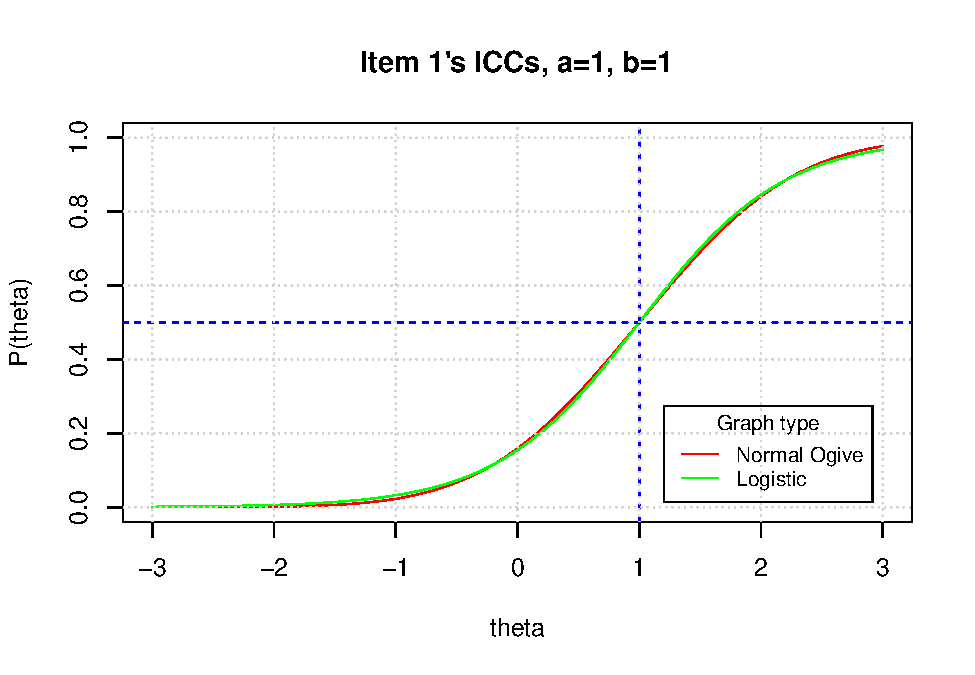
\includegraphics{Assignment_1_files/figure-latex/unnamed-chunk-8-1.pdf}
Now, the two ICCs are pretty close to each other.\\
Item 2 will have the same phenomenon, I skip plotting the item 2 for
space saving.

\hypertarget{q2-parta}{%
\subsection{Q2-Part(a)}\label{q2-parta}}

\emph{Plot the ICCs of the five items in the \ldots{}}

\textbf{My Solution: }\\
Using the function created above to plot five ICCs on one plot. Logistic
model with converted \(\alpha\) is used. I use 1PL model since the
discrimination information is not mentioned.

\begin{Shaded}
\begin{Highlighting}[]
\SpecialCharTok{\textgreater{}} \CommentTok{\# define the beta vector as input}
\ErrorTok{\textgreater{}}\NormalTok{ B }\OtherTok{\textless{}{-}} \FunctionTok{c}\NormalTok{(}\SpecialCharTok{{-}}\DecValTok{2}\NormalTok{, }\SpecialCharTok{{-}}\DecValTok{1}\NormalTok{, }\SpecialCharTok{{-}}\FloatTok{0.5}\NormalTok{, }\FloatTok{0.5}\NormalTok{, }\DecValTok{1}\NormalTok{)}
\SpecialCharTok{\textgreater{}} 
\ErrorTok{\textgreater{}} \CommentTok{\# using a for loop to get all results}
\ErrorTok{\textgreater{}}\NormalTok{ Ps }\OtherTok{\textless{}{-}} \FunctionTok{list}\NormalTok{()}
\SpecialCharTok{\textgreater{}} \ControlFlowTok{for}\NormalTok{ (i }\ControlFlowTok{in} \DecValTok{1}\SpecialCharTok{:}\FunctionTok{length}\NormalTok{(B))\{}
\SpecialCharTok{+}   \CommentTok{\# note a is a constant with value of 1.702 in 1PL model.}
\SpecialCharTok{+}\NormalTok{   P\_item1\_logit }\OtherTok{\textless{}{-}} \FunctionTok{logit\_2pl}\NormalTok{(}\AttributeTok{theta=}\NormalTok{theta,}\AttributeTok{a=}\FloatTok{1.702}\NormalTok{,}\AttributeTok{b=}\NormalTok{B[i])}
\SpecialCharTok{+}   \CommentTok{\# store the result into a list}
\SpecialCharTok{+}\NormalTok{   Ps[[i]] }\OtherTok{\textless{}{-}}\NormalTok{ P\_item1\_logit}
\SpecialCharTok{+}\NormalTok{ \}}
\SpecialCharTok{\textgreater{}} 
\ErrorTok{\textgreater{}} \CommentTok{\# plot all five ICCs on same plot}
\ErrorTok{\textgreater{}} \CommentTok{\# replot the two ICCs}
\ErrorTok{\textgreater{}} \FunctionTok{plot}\NormalTok{(theta, Ps[[}\DecValTok{1}\NormalTok{]], }\AttributeTok{type =} \StringTok{"l"}\NormalTok{, }
\SpecialCharTok{+}      \AttributeTok{col=}\StringTok{"red"}\NormalTok{, }\AttributeTok{xlim =} \FunctionTok{c}\NormalTok{(xlim\_min,xlim\_max), }\AttributeTok{ylim =} \FunctionTok{c}\NormalTok{(}\DecValTok{0}\NormalTok{,}\DecValTok{1}\NormalTok{),}
\SpecialCharTok{+}      \AttributeTok{main =} \StringTok{"5 ICCs using 1pl logistic model"}\NormalTok{, }\AttributeTok{ylab =} \StringTok{"P(theta)"}\NormalTok{)}
\SpecialCharTok{\textgreater{}} \CommentTok{\# using a for loop to plot the rest 4 ICCs}
\ErrorTok{\textgreater{}} \ControlFlowTok{for}\NormalTok{ (i }\ControlFlowTok{in} \FunctionTok{c}\NormalTok{(}\DecValTok{2}\SpecialCharTok{:}\DecValTok{5}\NormalTok{)) \{}
\SpecialCharTok{+}   \FunctionTok{lines}\NormalTok{(theta, Ps[[i]], }\AttributeTok{col=}\StringTok{"red"}\NormalTok{)}
\SpecialCharTok{+}\NormalTok{ \}}
\SpecialCharTok{\textgreater{}} \FunctionTok{abline}\NormalTok{(}\AttributeTok{h=}\FloatTok{0.5}\NormalTok{, }\AttributeTok{col=}\StringTok{"blue"}\NormalTok{, }\AttributeTok{lty=}\DecValTok{2}\NormalTok{)}
\SpecialCharTok{\textgreater{}} \FunctionTok{grid}\NormalTok{()}
\end{Highlighting}
\end{Shaded}

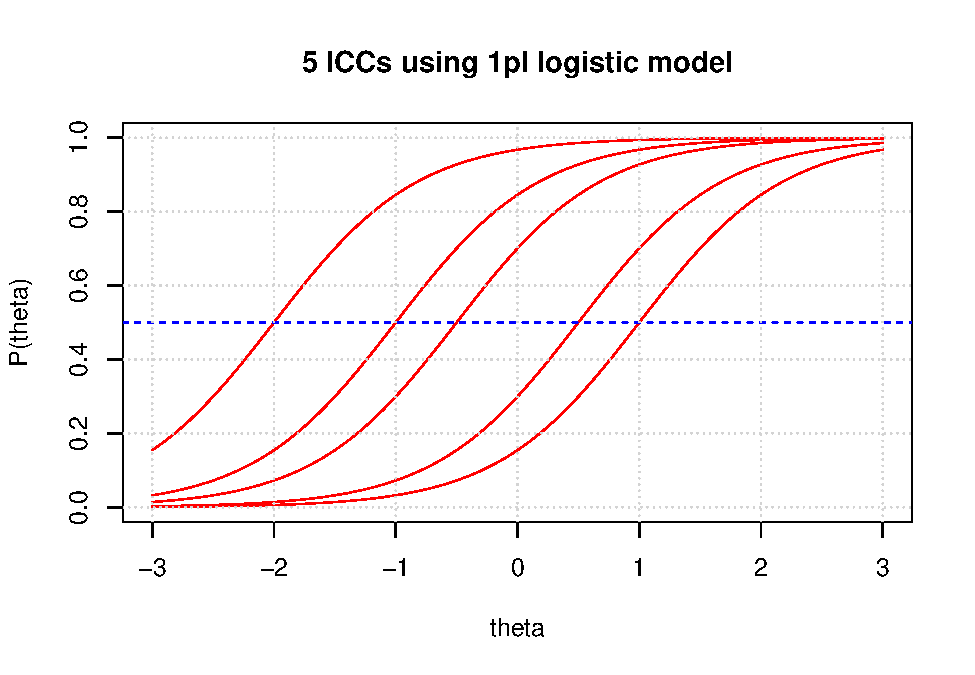
\includegraphics{Assignment_1_files/figure-latex/unnamed-chunk-9-1.pdf}

\hypertarget{q2-partb}{%
\subsection{Q2-Part(b)}\label{q2-partb}}

\emph{Compare the probabilities of correct response for Items \ldots{}}

\textbf{My Solution: }

For this 1PL model, item 1 (\(\beta=-2\)) is easier than item 4
(\(\beta=0.5\)). For example, for an examinee with trait level of 0
(i.e., \(\theta = 0\)), the probabilities to correctly answer the item 1
is around \(.96\) and around \(.3\) for item 4. Same phenomenon can be
also found for the examinees with a shared trait level across the trait
range \([-3,3]\). However, at the two extreme ends (i.e., the negative
infinity and the positive infinity), the probabilities should be same,
either 0 or 1.

\hypertarget{q2-partc}{%
\subsection{Q2-Part(c)}\label{q2-partc}}

\emph{Which of the five items is easiest \ldots{}}

\textbf{My Solution: }\\
The easiest item is item 1, and the item 5 is the most difficult. Yes.
By definition, the diffculty is an item's characteristic conditional on
\(\theta\). Therefore, Are these statements true for all \(\theta\).

\hypertarget{q2-partd}{%
\subsection{Q2-Part(d)}\label{q2-partd}}

\emph{Find TCC and Plot TCC \ldots{}}

\textbf{My Solution: }\\
By defintion, the TCC is sum of the \(P(\theta_j)\) for all items.

\begin{Shaded}
\begin{Highlighting}[]
\SpecialCharTok{\textgreater{}} \CommentTok{\# get the sum of all P\_thetas}
\ErrorTok{\textgreater{}}\NormalTok{ P\_tcc }\OtherTok{\textless{}{-}}\NormalTok{ Ps[[}\DecValTok{1}\NormalTok{]] }\SpecialCharTok{+}\NormalTok{ Ps[[}\DecValTok{2}\NormalTok{]] }\SpecialCharTok{+}\NormalTok{ Ps[[}\DecValTok{3}\NormalTok{]] }\SpecialCharTok{+}\NormalTok{ Ps[[}\DecValTok{4}\NormalTok{]] }\SpecialCharTok{+}\NormalTok{ Ps[[}\DecValTok{5}\NormalTok{]]}
\SpecialCharTok{\textgreater{}} 
\ErrorTok{\textgreater{}} \CommentTok{\# plot the TCC across thetas}
\ErrorTok{\textgreater{}} \FunctionTok{plot}\NormalTok{(theta, P\_tcc, }\AttributeTok{type =} \StringTok{"l"}\NormalTok{, }
\SpecialCharTok{+}      \AttributeTok{col=}\StringTok{"red"}\NormalTok{, }\AttributeTok{xlim =} \FunctionTok{c}\NormalTok{(xlim\_min,xlim\_max), }\AttributeTok{ylim =} \FunctionTok{c}\NormalTok{(}\DecValTok{0}\NormalTok{,}\DecValTok{6}\NormalTok{),}
\SpecialCharTok{+}      \AttributeTok{main =} \StringTok{"TCC"}\NormalTok{, }\AttributeTok{ylab =} \StringTok{"P(theta)"}\NormalTok{)}
\SpecialCharTok{\textgreater{}} \FunctionTok{abline}\NormalTok{(}\AttributeTok{v=}\SpecialCharTok{{-}}\DecValTok{1}\NormalTok{, }\AttributeTok{col=}\StringTok{"blue"}\NormalTok{, }\AttributeTok{lty=}\DecValTok{2}\NormalTok{)}
\SpecialCharTok{\textgreater{}} \FunctionTok{abline}\NormalTok{(}\AttributeTok{v=}\DecValTok{1}\NormalTok{, }\AttributeTok{col=}\StringTok{"blue"}\NormalTok{, }\AttributeTok{lty=}\DecValTok{2}\NormalTok{)}
\SpecialCharTok{\textgreater{}} \FunctionTok{grid}\NormalTok{()}
\end{Highlighting}
\end{Shaded}

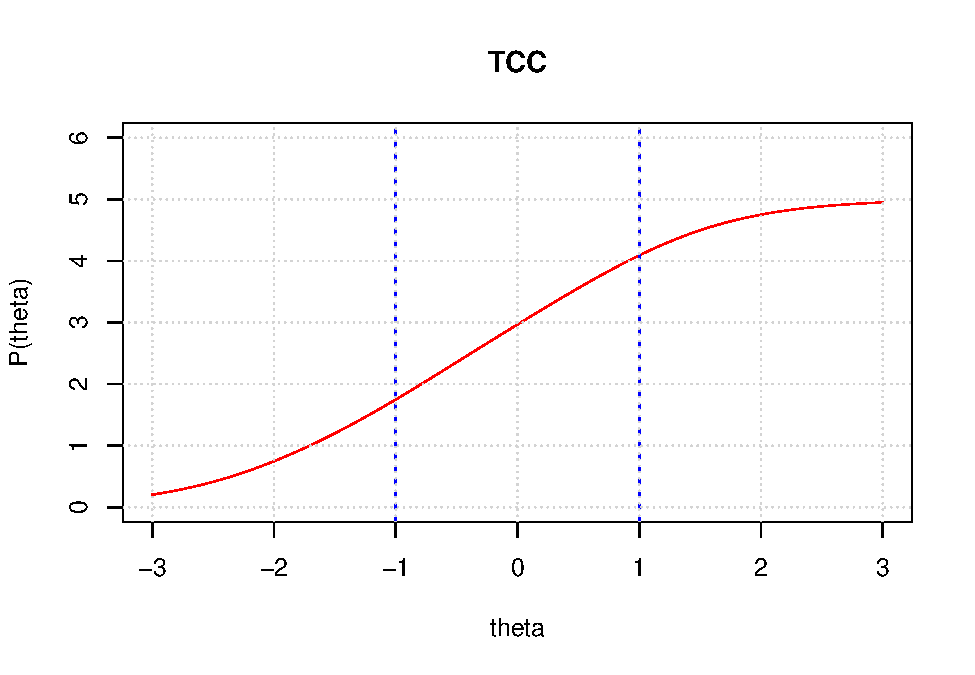
\includegraphics{Assignment_1_files/figure-latex/unnamed-chunk-10-1.pdf}

\hypertarget{q2-parte}{%
\subsection{Q2-Part(e)}\label{q2-parte}}

\emph{TCC also represents the expected number of correct responses
\ldots{}}

\textbf{My Solution: }\\
From the plot above, one might expect an examinee with the trait
\(\theta=-1.0\) to correctly answer around \(1.9\) items, and above
\(4\) items for an examinee with the trait at \(\theta=1\).

\hypertarget{q3-parta}{%
\subsection{Q3-Part(a)}\label{q3-parta}}

\emph{Find the mean of Item 6 and its correlation with \ldots{}}

\textbf{My Solution: }

For group 1, the difficulty(easiness) is \(.510\) and the discrimination
(using point bi-serial) is \(.276\).\\
For group 2, the difficulty(easiness) is \(.670\) and the discrimination
is \(.553\).

\hypertarget{q3-partb}{%
\subsection{Q3-Part(b)}\label{q3-partb}}

\emph{Do the indices remain the same across the two groups \ldots{}}

\textbf{My Solution: }\\
The indices are not the same across the groups. Since one limitation of
CTT is sample-dependent. Different sample will return different item
characteristics. CTT does not guarantee a indices invariance.

\hypertarget{q3-partc}{%
\subsection{Q3-Part(c)}\label{q3-partc}}

\emph{Which group has higher ability \ldots{}}

\textbf{My Solution: }

The Group 2's ability is greater than Group 1 since the average total
score is higher in Group 2.

\hypertarget{q4}{%
\subsection{Q4}\label{q4}}

\emph{Responses to three items at a fixed ability level can be \ldots{}}

\textbf{My Solution: }\\
The contingency tables for each pair as followed:\\
\includegraphics[width=0.5\textwidth,height=\textheight]{"q4.png"}

Next, I use the built-in function in R to conduct the \(\chi^2\) test.
Note, the null hypothesis of \(\chi^2\) test is that the variables are
independent.

\begin{Shaded}
\begin{Highlighting}[]
\SpecialCharTok{\textgreater{}} \CommentTok{\# load the data}
\ErrorTok{\textgreater{}}\NormalTok{ df }\OtherTok{\textless{}{-}} \FunctionTok{read.csv}\NormalTok{(}\StringTok{"\textasciitilde{}/Desktop/PhD\_Learning/HUDM6052 Psychometric II/assignment 1/hw1\_4.csv"}\NormalTok{)  }
\SpecialCharTok{\textgreater{}} 
\ErrorTok{\textgreater{}} \CommentTok{\# chi{-}square test for item 1 and 2}
\ErrorTok{\textgreater{}}\NormalTok{ result\_12 }\OtherTok{\textless{}{-}} \FunctionTok{chisq.test}\NormalTok{(}\FunctionTok{table}\NormalTok{(df[,}\FunctionTok{c}\NormalTok{(}\DecValTok{1}\NormalTok{,}\DecValTok{2}\NormalTok{)]))}
\SpecialCharTok{\textgreater{}}\NormalTok{ result\_13 }\OtherTok{\textless{}{-}} \FunctionTok{chisq.test}\NormalTok{(}\FunctionTok{table}\NormalTok{(df[,}\FunctionTok{c}\NormalTok{(}\DecValTok{1}\NormalTok{,}\DecValTok{3}\NormalTok{)]))}
\SpecialCharTok{\textgreater{}}\NormalTok{ result\_23 }\OtherTok{\textless{}{-}} \FunctionTok{chisq.test}\NormalTok{(}\FunctionTok{table}\NormalTok{(df[,}\FunctionTok{c}\NormalTok{(}\DecValTok{2}\NormalTok{,}\DecValTok{3}\NormalTok{)]))}
\SpecialCharTok{\textgreater{}}\NormalTok{ (pvalue\_12 }\OtherTok{\textless{}{-}}\NormalTok{ result\_12}\SpecialCharTok{$}\NormalTok{p.value)}
\NormalTok{[}\DecValTok{1}\NormalTok{] }\FloatTok{6.627178e{-}05}
\SpecialCharTok{\textgreater{}}\NormalTok{ (pvalue\_13 }\OtherTok{\textless{}{-}}\NormalTok{ result\_13}\SpecialCharTok{$}\NormalTok{p.value)}
\NormalTok{[}\DecValTok{1}\NormalTok{] }\FloatTok{0.7254943}
\SpecialCharTok{\textgreater{}}\NormalTok{ (pvalue\_23 }\OtherTok{\textless{}{-}}\NormalTok{ result\_23}\SpecialCharTok{$}\NormalTok{p.value)}
\NormalTok{[}\DecValTok{1}\NormalTok{] }\FloatTok{0.0001692519}
\end{Highlighting}
\end{Shaded}

The p-values from both tests of pair 1 (item 1 and item 2) and pair 3
(item 2 and item 3) are significant (\(\alpha\) = .05), which means
there are associations in both two pairs. Therefore, the local
independent assumption does not hold for item 1 and 2 and for item item
2 and item 3. Only item 1 and item 3 are locally independent.

\hypertarget{q5}{%
\subsection{Q5}\label{q5}}

\emph{Using the logistic model, plot the following three items over the
range \ldots{}}

\textbf{My Solution: }\\
I continue to use the function \texttt{logit\_2pl()} created in the
first question since it can fit for both 1PL and 2PL model. I write a
new function for 3PL model as followed.

\begin{Shaded}
\begin{Highlighting}[]
\SpecialCharTok{\textgreater{}} \CommentTok{\# write 3PL function}
\ErrorTok{\textgreater{}}\NormalTok{ logit\_3pl }\OtherTok{\textless{}{-}} \ControlFlowTok{function}\NormalTok{(theta, a, b, c)\{}
\SpecialCharTok{+}   \CommentTok{\# get the logit}
\SpecialCharTok{+}\NormalTok{   Z }\OtherTok{\textless{}{-}}\NormalTok{ a}\SpecialCharTok{*}\NormalTok{(theta}\SpecialCharTok{{-}}\NormalTok{b)}
\SpecialCharTok{+}   \CommentTok{\# get the probability}
\SpecialCharTok{+}\NormalTok{   P }\OtherTok{\textless{}{-}}\NormalTok{ c }\SpecialCharTok{+}\NormalTok{ (}\DecValTok{1}\SpecialCharTok{{-}}\NormalTok{c)}\SpecialCharTok{/}\NormalTok{(}\DecValTok{1} \SpecialCharTok{+} \FunctionTok{exp}\NormalTok{(}\SpecialCharTok{{-}}\NormalTok{Z))}
\SpecialCharTok{+}   \FunctionTok{return}\NormalTok{(P)}
\SpecialCharTok{+}\NormalTok{ \}}
\end{Highlighting}
\end{Shaded}

Then, I calculate the probability vector for each model.

\begin{Shaded}
\begin{Highlighting}[]
\SpecialCharTok{\textgreater{}} \CommentTok{\# for the 1Pl model, b=0.5}
\ErrorTok{\textgreater{}}\NormalTok{ P\_1pl }\OtherTok{\textless{}{-}} \FunctionTok{logit\_2pl}\NormalTok{(}\AttributeTok{theta=}\NormalTok{theta, }\AttributeTok{a=}\DecValTok{1}\NormalTok{, }\AttributeTok{b=}\FloatTok{0.5}\NormalTok{)}
\SpecialCharTok{\textgreater{}} \CommentTok{\# for the 2PL model, a=1.5, b=0.5}
\ErrorTok{\textgreater{}}\NormalTok{ P\_2pl }\OtherTok{\textless{}{-}} \FunctionTok{logit\_2pl}\NormalTok{(}\AttributeTok{theta =}\NormalTok{ theta, }\AttributeTok{a=}\FloatTok{1.5}\NormalTok{, }\AttributeTok{b=}\FloatTok{0.5}\NormalTok{)}
\SpecialCharTok{\textgreater{}} \CommentTok{\# for the 3PL model, a=1.5, b=0.5, c=0.15}
\ErrorTok{\textgreater{}}\NormalTok{ P\_3pl }\OtherTok{\textless{}{-}} \FunctionTok{logit\_3pl}\NormalTok{(}\AttributeTok{theta =}\NormalTok{ theta, }\AttributeTok{a=}\FloatTok{1.5}\NormalTok{, }\AttributeTok{b=}\FloatTok{0.5}\NormalTok{, }\AttributeTok{c=}\FloatTok{0.15}\NormalTok{)}
\end{Highlighting}
\end{Shaded}

Next, plot all 3 ICCs on same plot.

\begin{Shaded}
\begin{Highlighting}[]
\SpecialCharTok{\textgreater{}} \FunctionTok{plot}\NormalTok{(theta, P\_1pl, }\AttributeTok{type =} \StringTok{"l"}\NormalTok{, }
\SpecialCharTok{+}      \AttributeTok{col=}\StringTok{"red"}\NormalTok{, }\AttributeTok{xlim =} \FunctionTok{c}\NormalTok{(xlim\_min,xlim\_max), }\AttributeTok{ylim =} \FunctionTok{c}\NormalTok{(}\DecValTok{0}\NormalTok{,}\DecValTok{1}\NormalTok{),}
\SpecialCharTok{+}      \AttributeTok{main =} \StringTok{"ICCs for 3 Models"}\NormalTok{, }\AttributeTok{ylab =} \StringTok{"P(theta)"}\NormalTok{)}
\SpecialCharTok{\textgreater{}} \FunctionTok{lines}\NormalTok{(theta, P\_2pl, }\AttributeTok{col=}\StringTok{"darkgreen"}\NormalTok{)}
\SpecialCharTok{\textgreater{}} \FunctionTok{lines}\NormalTok{(theta, P\_3pl, }\AttributeTok{col=}\StringTok{"purple"}\NormalTok{)}
\SpecialCharTok{\textgreater{}} \FunctionTok{abline}\NormalTok{(}\AttributeTok{h=}\FloatTok{0.5}\NormalTok{, }\AttributeTok{col=}\StringTok{"blue"}\NormalTok{, }\AttributeTok{lty=}\DecValTok{2}\NormalTok{)}
\SpecialCharTok{\textgreater{}} \FunctionTok{abline}\NormalTok{(}\AttributeTok{h=}\FloatTok{0.575}\NormalTok{, }\AttributeTok{col=}\StringTok{"blue"}\NormalTok{, }\AttributeTok{lty=}\DecValTok{2}\NormalTok{)}
\SpecialCharTok{\textgreater{}} \FunctionTok{grid}\NormalTok{()}
\SpecialCharTok{\textgreater{}} \CommentTok{\# add legend}
\ErrorTok{\textgreater{}} \FunctionTok{legend}\NormalTok{(}\StringTok{\textquotesingle{}bottomright\textquotesingle{}}\NormalTok{,}\AttributeTok{inset=}\FloatTok{0.05}\NormalTok{,}
\SpecialCharTok{+}        \FunctionTok{c}\NormalTok{(}\StringTok{"1PL"}\NormalTok{,}\StringTok{"2PL"}\NormalTok{,}\StringTok{"3PL"}\NormalTok{),}\AttributeTok{lty=}\DecValTok{1}\NormalTok{,}
\SpecialCharTok{+}        \AttributeTok{col=}\FunctionTok{c}\NormalTok{(}\StringTok{"red"}\NormalTok{,}\StringTok{"darkgreen"}\NormalTok{,}\StringTok{"purple"}\NormalTok{),}\AttributeTok{title=}\StringTok{"Graph type"}\NormalTok{,}
\SpecialCharTok{+}        \AttributeTok{cex=}\FloatTok{0.8}\NormalTok{)}
\end{Highlighting}
\end{Shaded}

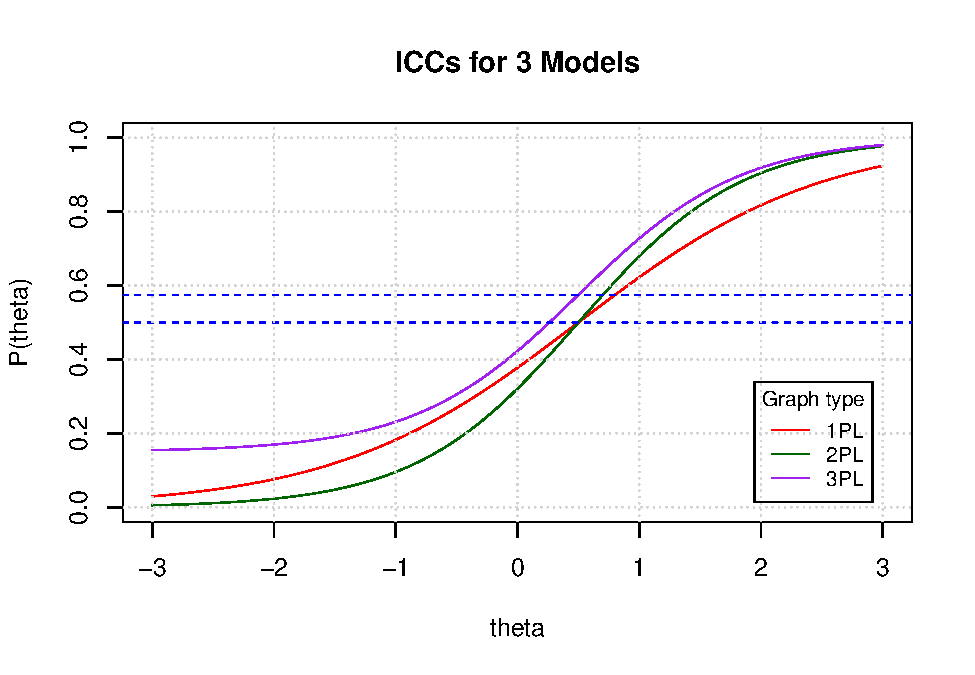
\includegraphics{Assignment_1_files/figure-latex/unnamed-chunk-14-1.pdf}

\hypertarget{q6}{%
\subsection{Q6}\label{q6}}

\emph{For the three-parameter logistic model \ldots{}}

\textbf{My Solution: }\\
By definition, the 3PL model is
\[P(\theta)= c+ (1-c)\frac{1}{1+e^{-\alpha(\theta-\beta)}} .\]\\
Set the \(\theta = \beta\), we have
\[P(\theta = \beta)= c+ (1-c)\frac{1}{1+e^0} .\]\\
Since the \(e^0 = 1\), finally, we have
\[P(\theta = \beta)= c+ (1-c)\frac{1}{2}=\frac{1}{2} (1+c) .\]

\end{document}
